\chapter{Introduction}
\label{ch:introduction}

\section{Project Overview}
\label{sec:project_overview}

The Vehicle Tracking System represents a comprehensive, real-time GPS fleet management solution engineered using the \flutter{} framework and \firebase{} backend services. This system delivers live vehicle monitoring, driver behavior analysis, route optimization, and advanced reporting capabilities across multiple platforms including mobile, web, and desktop applications.

\begin{figure}[H]
    \centering
    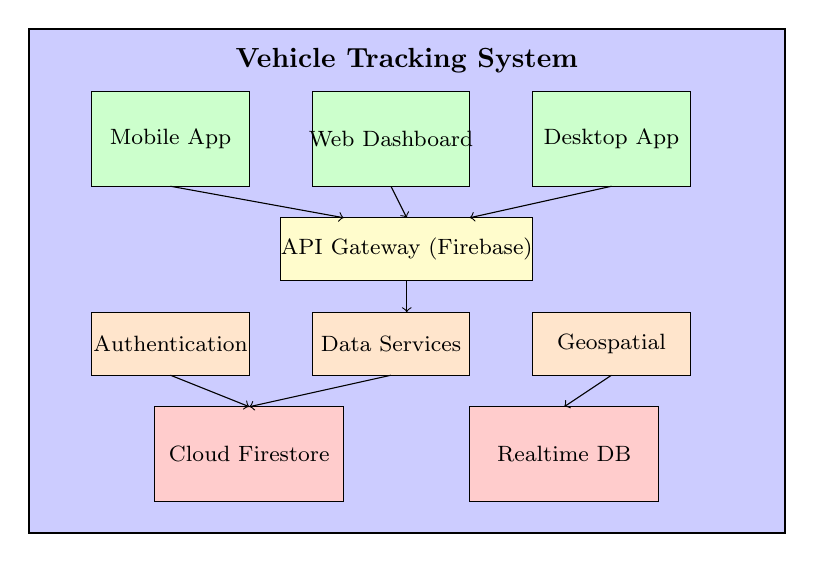
\begin{tikzpicture}[scale=0.8]
        % System overview diagram
        \draw[thick, fill=blue!20] (0,0) rectangle (12,8);
        \node at (6,7.5) {\textbf{Vehicle Tracking System}};
        
        % Client layer
        \draw[fill=green!20] (1,5.5) rectangle (3.5,7);
        \node at (2.25,6.25) {\footnotesize Mobile App};
        
        \draw[fill=green!20] (4.5,5.5) rectangle (7,7);
        \node at (5.75,6.25) {\footnotesize Web Dashboard};
        
        \draw[fill=green!20] (8,5.5) rectangle (10.5,7);
        \node at (9.25,6.25) {\footnotesize Desktop App};
        
        % API Gateway
        \draw[fill=yellow!20] (4,4) rectangle (8,5);
        \node at (6,4.5) {\footnotesize API Gateway (Firebase)};
        
        % Backend services
        \draw[fill=orange!20] (1,2.5) rectangle (3.5,3.5);
        \node at (2.25,3) {\footnotesize Authentication};
        
        \draw[fill=orange!20] (4.5,2.5) rectangle (7,3.5);
        \node at (5.75,3) {\footnotesize Data Services};
        
        \draw[fill=orange!20] (8,2.5) rectangle (10.5,3.5);
        \node at (9.25,3) {\footnotesize Geospatial};
        
        % Database layer
        \draw[fill=red!20] (2,0.5) rectangle (5,2);
        \node at (3.5,1.25) {\footnotesize Cloud Firestore};
        
        \draw[fill=red!20] (7,0.5) rectangle (10,2);
        \node at (8.5,1.25) {\footnotesize Realtime DB};
        
        % Arrows
        \draw[->] (2.25,5.5) -- (5,5);
        \draw[->] (5.75,5.5) -- (6,5);
        \draw[->] (9.25,5.5) -- (7,5);
        \draw[->] (6,4) -- (6,3.5);
        \draw[->] (2.25,2.5) -- (3.5,2);
        \draw[->] (5.75,2.5) -- (3.5,2);
        \draw[->] (9.25,2.5) -- (8.5,2);
    \end{tikzpicture}
    \caption{Vehicle Tracking System High-Level Architecture}
    \label{fig:system_overview}
\end{figure}

\section{Project Background}
\label{sec:project_background}

The transportation and logistics industry has experienced unprecedented growth, driven by e-commerce expansion and globalization. Traditional vehicle tracking methods have proven inadequate for modern business requirements, necessitating intelligent, real-time solutions that can adapt to dynamic operational needs.

\subsection{Market Context}
The global vehicle tracking system market, valued at USD 2.94 billion in 2022, is projected to reach USD 6.04 billion by 2030, exhibiting a CAGR of 9.4\% during the forecast period \cite{market_research_2023}. This growth is attributed to:

\begin{itemize}
    \item Increasing demand for fleet optimization and fuel cost reduction
    \item Growing emphasis on driver safety and behavior monitoring
    \item Rising adoption of IoT and cloud-based solutions
    \item Regulatory requirements for commercial vehicle monitoring
\end{itemize}

\subsection{Technology Evolution}
The evolution of mobile technologies has created unprecedented opportunities for developing sophisticated tracking solutions:

\begin{table}[H]
    \centering
    \caption{Technology Evolution in Vehicle Tracking}
    \label{tab:tech_evolution}
    \begin{tabular}{@{}llll@{}}
        \toprule
        \textbf{Generation} & \textbf{Technology} & \textbf{Capabilities} & \textbf{Limitations} \\
        \midrule
        1st Gen & GPS + GSM & Basic location tracking & High latency, limited features \\
        2nd Gen & GPS + 3G & Real-time updates & Expensive, complex integration \\
        3rd Gen & Smartphone-based & Multi-platform apps & Battery dependency \\
        4th Gen & Cloud-native & Real-time analytics & Requires internet connectivity \\
        \bottomrule
    \end{tabular}
\end{table}

\section{Problem Domain}
\label{sec:problem_domain}

The transportation and logistics industry confronts several critical challenges that traditional tracking systems fail to address adequately:

\subsection{Operational Inefficiencies}
\begin{enumerate}
    \item \textbf{Limited Real-time Visibility}: Traditional systems provide updates with significant delays (5-15 minutes), hindering real-time decision making.
    \item \textbf{Fragmented Data Systems}: Multiple disconnected platforms create operational silos and increase administrative overhead.
    \item \textbf{Poor Route Optimization}: Manual route planning leads to increased fuel consumption and delivery delays.
\end{enumerate}

\subsection{Technical Limitations}
\begin{enumerate}
    \item \textbf{Scalability Constraints}: Legacy systems struggle with growing fleet sizes and increasing data volumes.
    \item \textbf{Integration Challenges}: Limited API access and poor documentation complicate system integration.
    \item \textbf{Mobile User Experience}: Most solutions prioritize web interfaces over mobile optimization.
\end{enumerate}

\section{Solution Approach}
\label{sec:solution_approach}

Our Vehicle Tracking System addresses these challenges through a comprehensive approach leveraging modern technologies:

\subsection{Core Innovations}
\begin{description}
    \item[Real-time Architecture] Utilizing \firebase{} Realtime Database for sub-30-second location updates
    \item[Cross-platform Consistency] Single \flutter{} codebase ensuring identical functionality across platforms
    \item[Cloud-native Design] Serverless architecture enabling automatic scaling and cost optimization
    \item[Mobile-first Approach] Optimized user experience for mobile users with web as secondary interface
\end{description}

\subsection{Technical Advantages}
The system incorporates several technical innovations:

\begin{lstlisting}[language=Dart, caption={Real-time Location Update Implementation}, label={lst:realtime_update}]
class LocationService {
  static const Duration _updateInterval = Duration(seconds: 30);
  
  Stream<Position> getLocationStream() {
    return Geolocator.getPositionStream(
      locationSettings: LocationSettings(
        accuracy: LocationAccuracy.high,
        distanceFilter: 10, // meters
        timeLimit: _updateInterval,
      ),
    );
  }
  
  Future<void> updateRealtimeLocation(
    String vehicleId, 
    LocationModel location
  ) async {
    await FirebaseDatabase.instance
        .ref('live_tracking/$vehicleId')
        .set({
      'latitude': location.latitude,
      'longitude': location.longitude,
      'timestamp': ServerValue.timestamp,
      'speed': location.speed,
      'heading': location.heading,
    });
  }
}
\end{lstlisting}

\section{Key Stakeholders}
\label{sec:stakeholders}

The system serves multiple stakeholder groups with distinct requirements:

\subsection{Primary Users}
\begin{description}
    \item[Fleet Managers] System administrators responsible for overall fleet operations and strategic decision-making
    \item[Drivers] Mobile app users providing location data and receiving navigation assistance
    \item[Dispatchers] Personnel responsible for real-time monitoring and route optimization
    \item[Business Owners] Executive dashboard users requiring high-level analytics and ROI metrics
\end{description}

\subsection{Secondary Users}
\begin{description}
    \item[Maintenance Teams] Personnel responsible for vehicle health monitoring and maintenance scheduling
    \item[Customers] End recipients requiring delivery tracking and estimated time of arrival (ETA) information
    \item[Regulatory Bodies] Organizations requiring compliance reporting and audit capabilities
\end{description}

\section{Document Organization}
\label{sec:document_organization}

This technical documentation is structured to provide comprehensive coverage of the Vehicle Tracking System development:

\begin{description}
    \item[Chapter \ref{ch:literature_review}] Examines existing solutions and identifies research gaps
    \item[Chapter \ref{ch:problem_statement}] Details problem definition and requirements analysis
    \item[Chapter \ref{ch:objectives}] Establishes project goals and success criteria
    \item[Chapter \ref{ch:methodology}] Outlines development methodologies and processes
    \item[Chapter \ref{ch:system_architecture}] Presents technical architecture and design decisions
    \item[Chapter \ref{ch:implementation}] Details implementation specifics and code examples
    \item[Chapter \ref{ch:testing}] Describes testing strategies and quality assurance
    \item[Chapter \ref{ch:results}] Analyzes performance metrics and system evaluation
    \item[Chapter \ref{ch:future_scope}] Discusses enhancement opportunities and roadmap
\end{description}

The documentation follows IEEE standards for technical documentation and incorporates academic research methodologies to ensure comprehensive coverage and reproducibility of results.
